%!TEX root = Manuscript.tex

\chapter{Proof of feasibility}
\label{chap:TSN}
\minitoc

In this thesis, we proposed algorithms that minimize contention in several kinds of networks, either by removing buffers or computing mnimal buffering time. As we explained, it is necessary that packets are not or as little as possible delayed in the network. Delay causes are various, but the main one is the buffering time. 

Our approach of the network consists in managing the message in each node in order to keep the buffuring under control. This is related to the concept of Deterministic Networking. A working group from IETF called DetNet~\cite{finn-detnet-architecture-08} works in collaboration with TSN (Time Sensitive Networking)~\cite{ieee802}, a task group of IEEE, to develop technical solutions for deterministic networking. While DetNet works on Layer 3, TSN devlop solutions for Layer 2. Since our model is based on ethernet we focus on TSN standards.

This chapter introduce in Section~\ref{sec:TSNqbv} the IEEE standards for TSN that allows a better network managment based on scheduled packets and on which our model is based. TSN standards are designed to manage stochastic flows in network. Nevertheless, we show that managing deterministic traffic allows us to remove some technical constraint, and leads us to new technology, that we call Hyper-TSN. Section~\ref{sec:platform} present a prototype of a switch that goes beyond TSN, by delivering packet at exact expected dates without any additional latency or synchronization constraint. In Hyper TSN, the latency is as close as possible with physical limitations.


\section{A Customized Managment of the Network}
\label{sec:TSNqbv}

\subsection{Overview of TSN standards}
The model we present in Chapter~\ref{chap:model} is based on several assumption:
\begin{itemize}
\item The aglorithms we developped are based on a central knowledge of the network and suppose all nodes are able to follow instructions. There must be an entity that centralizes and manages the nodes.
\item We suppose that all nodes are perfectly synchronized on the same clock.
\item We suppose the nodes are able to distinguish and manage differently each flows.
\end{itemize}
We explain in this chapter how the recent standards developed by TSN task group connect to such a model. A detailled survey of all TSN standards can be found in~\cite{8458130}. 


The stadard IEEE 802.1Qat SRP~\cite{article} (Stream Rerservation Protocol) provides a central managment framework that allow a centralized entity to collect datas about the flows. It has been improved by IEEE 802.1Qcc~\cite{6755436}. Those standards a centralized entity, that we call \textbf{controller}, to collect all required informations needed by users about the network (the routing, the periodicity and the size of the datagrams). This controller proposes an user interface that allows users to collect all network informations in order to compute the configuration of the network. Figure~\ref{fig:networkcontroller} shows a network managed by a controller, communicating via its user interface with algorithms, and able to send requirement to the nodes. Such an approach is related to Softward Defined Network (SDN)~\cite{li2015software}. We can find in~\cite{7356556} an example of SDN for TSN.


\begin{figure}
\begin{center}
\scalebox{0.4}{

\begin{tikzpicture}
  \SetGraphUnit{5}
    \tikzset{
  EdgeStyle/.append style = {->} }
   \tikzstyle{VertexStyle}=[shape = circle, draw, minimum size = 30pt]
 

  \node (r1) at (0,0) {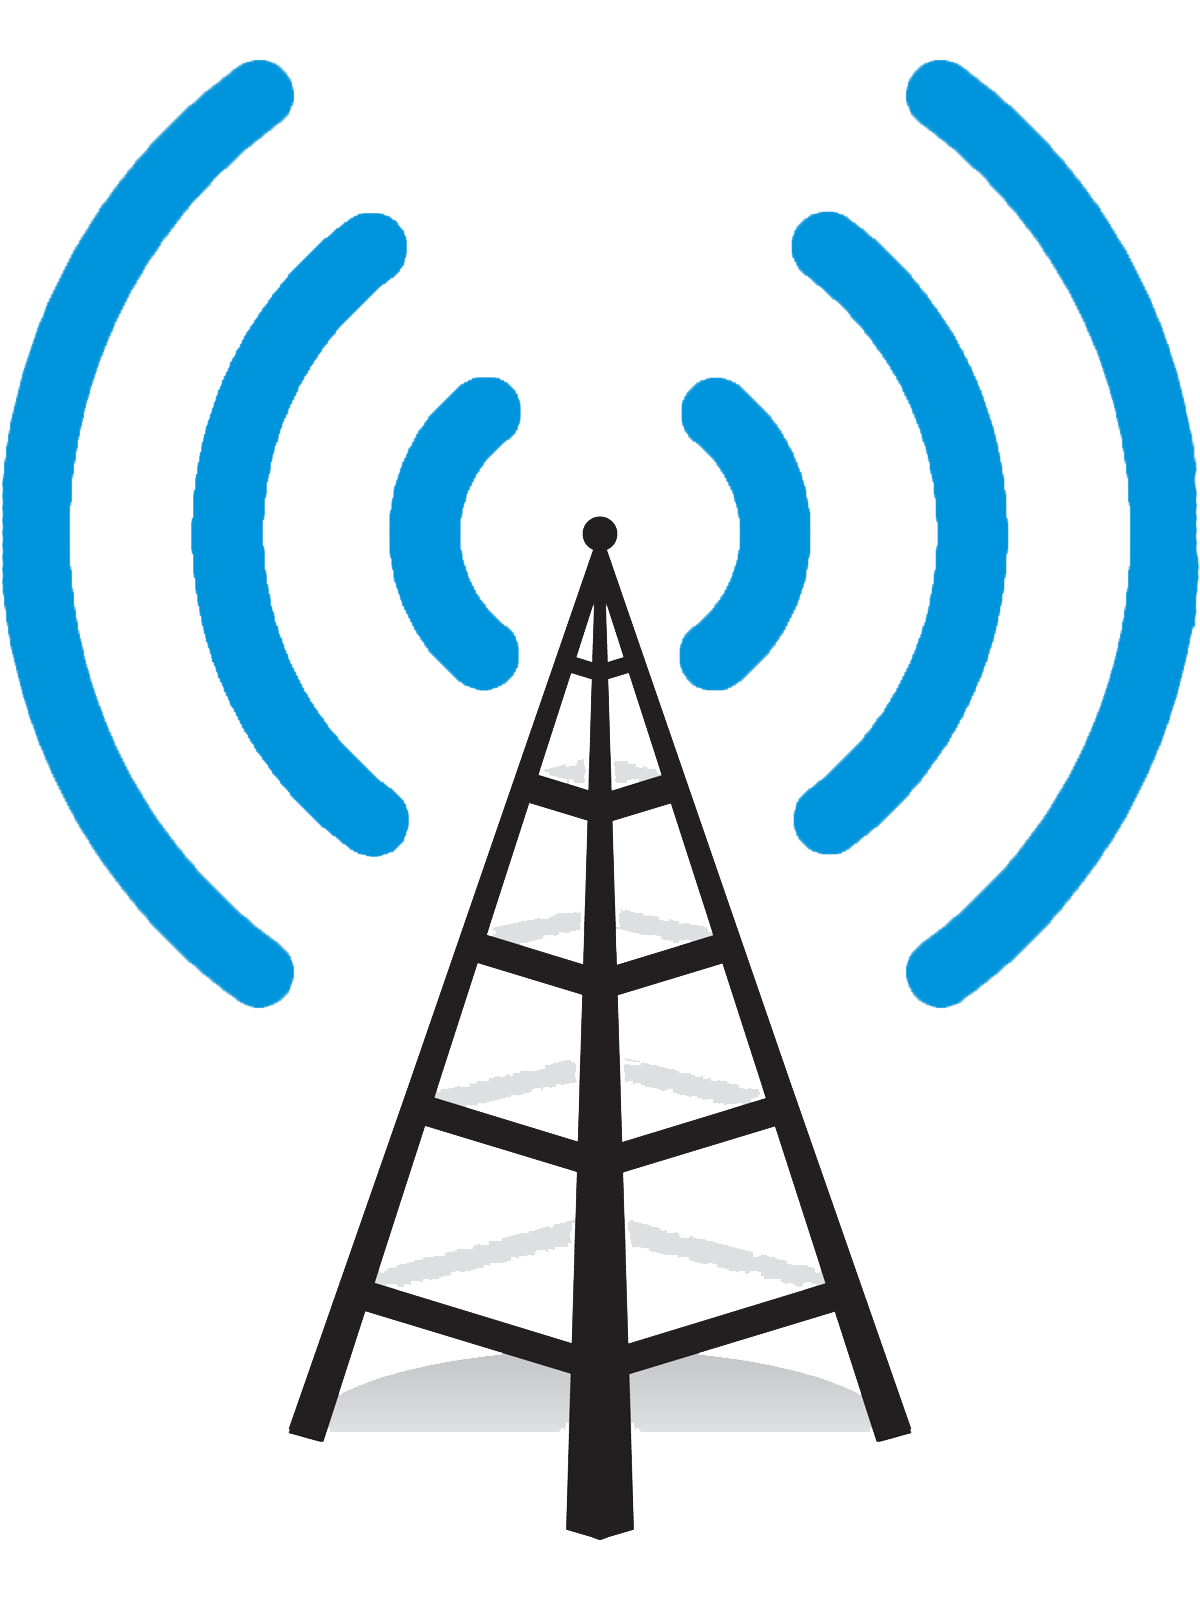
\includegraphics[width = 1cm]{rrh.png}};
   \node[below] at (r1.south) {RRH};
  \node (r2) at (0,4) {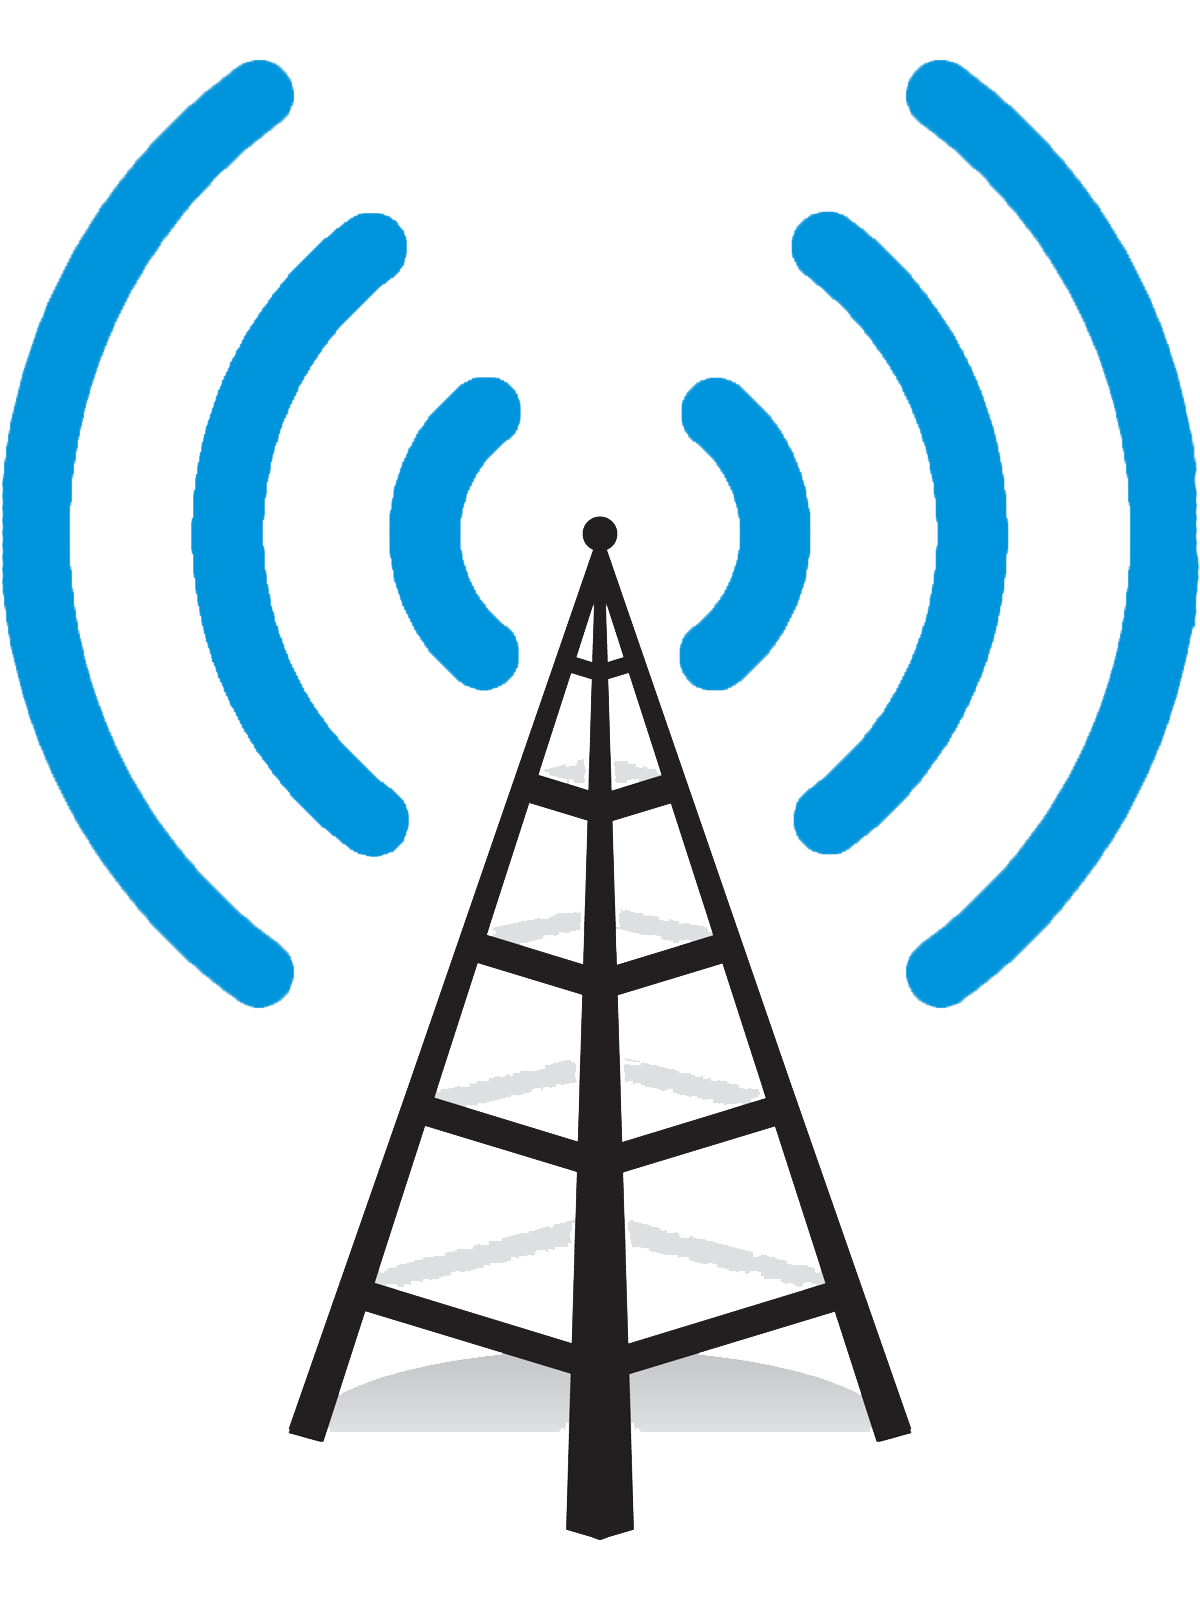
\includegraphics[width = 1cm]{rrh.png}};
   \node[below] at (r2.south) {RRH};
   \node (b1) at (12,0) {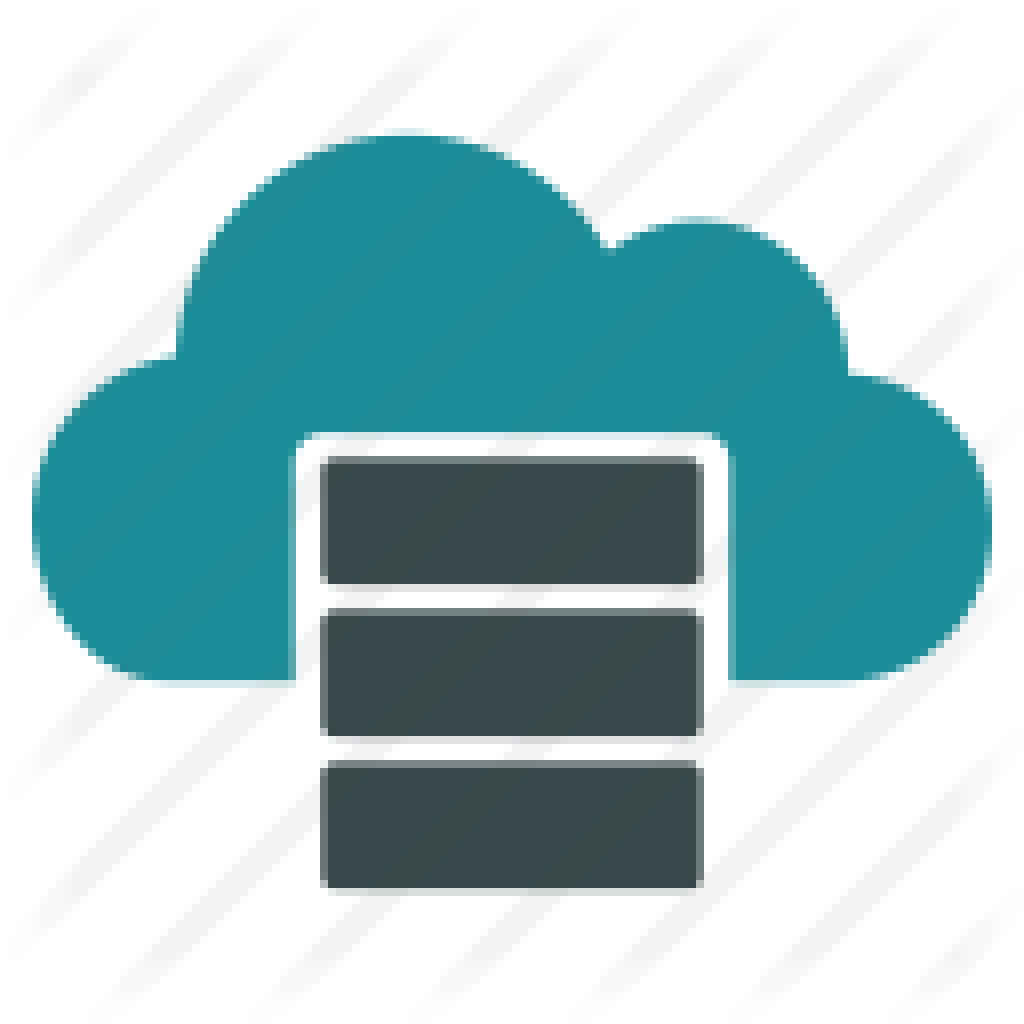
\includegraphics[width = 1cm]{bbu.png}};
   \node[below] at (b1.south) {BBU};
   \node (b2) at (12,4) {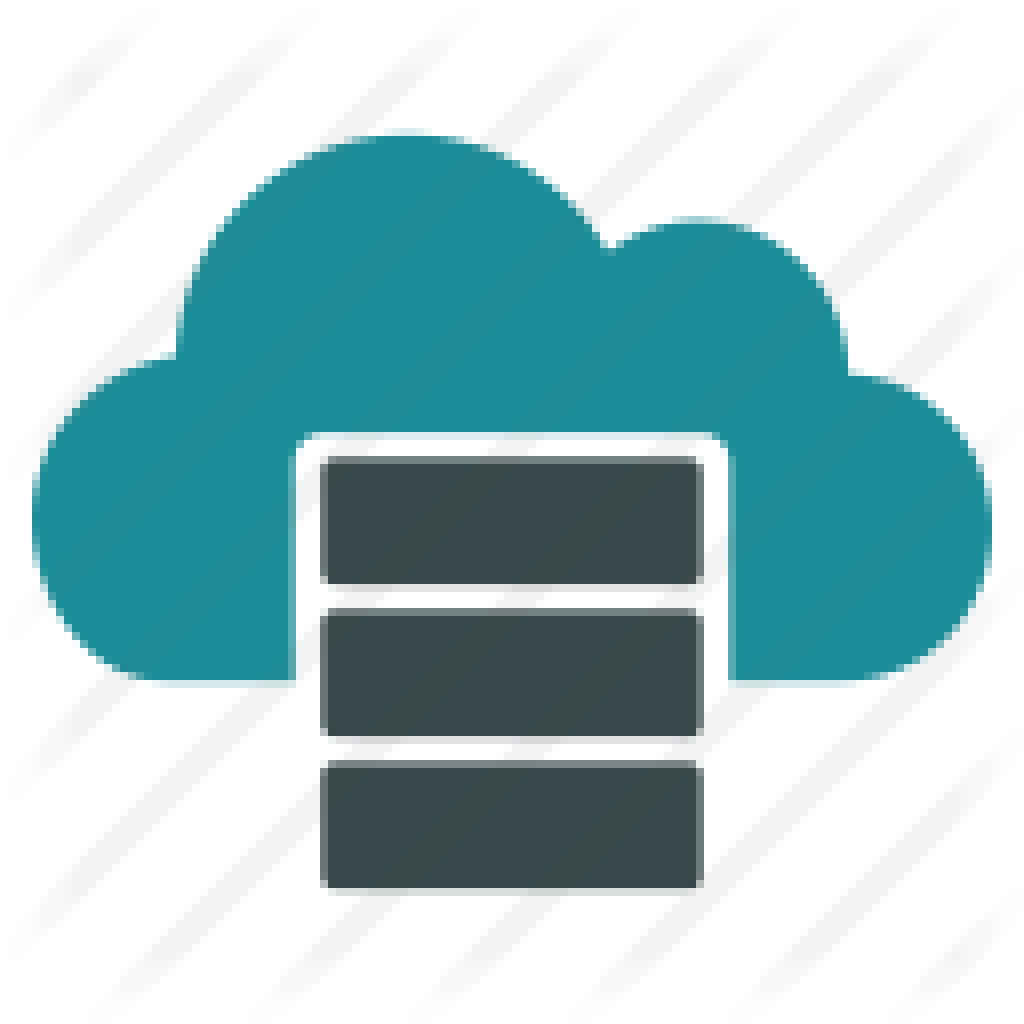
\includegraphics[width = 1cm]{bbu.png}};
	\node[below] at (b2.south) {BBU};
   \node (s1) at (4,2) {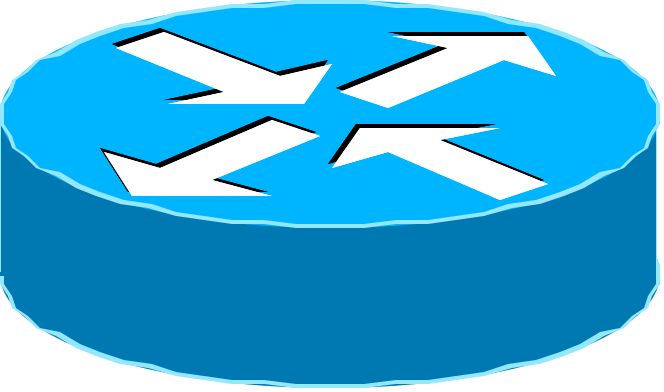
\includegraphics[width = 1cm]{switch.png}};
   \node (s2) at (8,2) {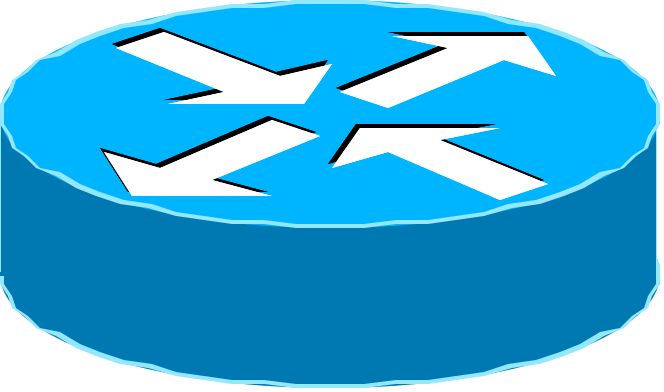
\includegraphics[width = 1cm]{switch.png}};
  
   \node (c) at (6,6) {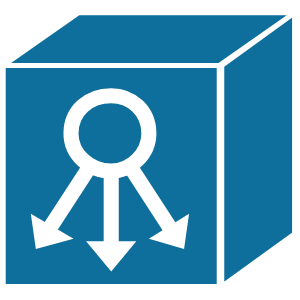
\includegraphics[width = 1cm]{controller.png}};
   	\node[right] at (c.north east) {Controller};

   	\node (rect) at (6,10) [draw,thick,minimum width=2cm,minimum height=1cm] {Algorithms};

\path (r1) edge [<->]  (s1);
\path (r2) edge [<->]  (s1);
\path (s2) edge [<->]  (s1);
\path (s2) edge [<->]  (b1);
\path (s2) edge [<->]  (b2);
\path (s2) edge [<->]  (c);
\path (s1) edge [<->]  (c);
\path (r1) edge [<->]  (c);
\path (r2) edge [<->]  (c);
\path (b1) edge [<->]  (c);
\path (b2) edge [<->]  (c);
\path (rect) edge [<->]  (c);


\end{tikzpicture}
}


 \caption{A TSN network managed by a cotroller, able to collect network informations, and control the nodes behavior.}

\label{fig:networkcontroller}
\end{center}
\end{figure}


Standard 802.1Qbv~\cite{8613095} allows us to manage differently flows in the nodes by a gate mechanism. The switch follows a routine that order to every node the date at which a flow must be sent on each output port. To do so, the switch needs a Gate Control List (GCL). This GCL is computed by the user, and sent to each switch of the network by the controller. It is a list of dates, and for every date of the list are specified the output ports (gates) of the switch which are open or close.


Figure~\ref{fig:tsnqbv} found in~\cite{durr2016no} shows the mechanism of a switch using 802.1Qbv technology. Considering a given period ($T_{cycle}$ in the figure), the switch selects at each time ($T_1 , T_2 , \ldots$ the queues that must be open to transmit packets. In figure 6, at time $T_1$, all gates except the one for scheduled traffic are open, at time $T_2$, all gates are closed and at time $T_3$ only the gate for scheduled traffic is open.

  \begin{figure}
  \begin{center}
  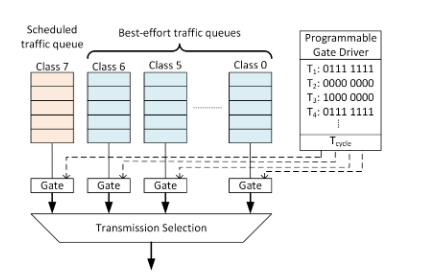
\includegraphics[width=0.8\textwidth]{Chapitre1/tsnqbv.png}
  \end{center}
  \caption{IEEE 802.1Qbv mechanism}\label{fig:tsnqbv}
  \end{figure}
      
With such a mechanism, it is possible organize the flows in order to control the latency. To do so, it is necessary to compute the CGL upstream. The GCL are computed considering the average traffic of each flow. Several works on Time Aware Shaping have been developed on this topic \todo{ref, reprendre}

To be efficient, the components of the network must completely synchronized. Such an hypothesis seems unrealistic, standards likes IEEE 802.1AS~\cite{5741898}, or IEEE 1588~\cite{4579760} propose good solutions for clock synchronization, but this problem is still difficult to solve. \todo{délai non connu a cause des changements de température}

\subsection{Limits of TSN when managing Deterministic flows}

All those standards are designed for a statistical managment of the flows. In this thesis, we work on deterministic flows. This means our models and computations are not made following a statistical approach like in current traffic shaping, but a deterministical approach: We are able to compute the exact date at wich each flow is able to reach each node. 

Such an approach requires to rethink about our vision of the network managment. We need the nodes to be perfectly synchronized otherwise it could be counter productive. Indeed, if a packet of a flow arrives in a node before or after the planned date, the gate is close and the packet is buffered, that induces additional latency.

Also, switches operation on the physical layer of the network induce an additional latency. In store-and-forward concept~\cite{tindell1992store}, packets are stored at reception of a node before being forwarded. However, solution like cut-through~\cite{kermani1979virtual} allow to reduce storage size and corresponding delay to the header size only. But this is effective if the egress port is available to forward the packet at the same time only. If not, the packet is buffered until the port get free. Even if it is possible to adapt our algorithm to take into consideration the physical delay cost, it still induce additional latency, which is not desirable.


\section{Deterministic managment for a deterministic latency}
\label{sec:platform}

\todo{dire que bcp de gens se disent "determinisite" alors qu'ils ne font que de la latence bornée.}
The problem we define is to manage deterministic flows. Hence, multiple standards of TSN are not usfeull yet. Indeed, since the exact date of arrival of all packets are computed, there is no point to manage the traffic on a statistical manner. 

We present in this section an Hyper-TSN switch that solves all the problematic of TSN when managing deterministic traffic.
This technology is under an advanced phase of research, and a prototype has been experimented in Nokia Bell Labs\todo{paper to be published}


\subsection{Hyper-TSN switch}


The main idea of such a switch is to take the flow as a reference. 

The synchronisation problem is solved by the monitoring and the


An Hyper-TSN switch has been developped. It is composed of a deterministic scheduler, two 10 Gbps ethernet ingress and two 10 Gbps ethernet egress ports. The deterministic scheduler is configured with a timing table. This table is similar to a 802,1 Qbv Gate Control List (GCL). It defines the periodicity of the scheduling and, for each port, the planed date of arrival of the datagrams. At each of these dates the deterministic scheduler sets the switch to transmit data incoming on a specified ingress port.

To perform experiments a generator of deterministic flows has been developed on a Xilinx FPGA board,Zynq-7000 SoC zc706. This generator offsets the dates it sends the frames according to the controls received from the monitoring circuitry.

To perform the experiment the generator is configured to send frames on both egress ports according to the period defined in the timing table. The size of the frames is set to fully load the ethernet links (ie $100\%$ load).

When starting, the monitoring circuitry detects that frames do not arrive at the planed date and sends control commands to the generator. These first frames are lost. Once the generator has rightly offset the dates it sends the frames, nor more offset has been performed during the running 2 hours experiment.

Then $100\%$ of the frames are correctly switched without being corrupted or lost. The switching of each frame from the ingress port to the planed egress port is performed introducing only one clock cycle delay (here 3,87 ns).
